


In this section, we evaluate the effectiveness of \textit{UniRel} on relation-centric KGQA across multiple datasets and LLMs.
We first describe the datasets and models, then present the main results, followed by analyses of generalization and scalability under multi-entity queries.
Finally, we apply the \textit{UniRel} pipeline to conventional entity-centric KGQA to assess its transferability.

\subsection{Experiment Setup}



\textbf{Datasets.} We evaluate on seven benchmark KG datasets to ensure diversity in scale, domain, and relational complexity:
Freebase13~\citep{Socher2013ReasoningWN}, FB15k-237~\citep{toutanova2015observed}, MetaQA~\citep{zhang2018variational},
DBpedia50/500~\citep{Auer07DBpedia}, YAGO3-10~\citep{Mahdisoltani2015YAGO3AK}, and UMLS~\citep{bodenreider2004umls}.
These datasets span encyclopedic, biomedical, and commonsense knowledge, providing a testbed for relation-centric KGQA.
Dataset statistics are reported in Appendix~\ref{sec:implement_details}.



\textbf{Query Construction.} Existing KGQA benchmarks focus on \textit{entity-centric} queries that return a single entity.  
To adapt them to the relation-centric setting, we constructed 2,500 queries per dataset, with 2,000 for training and 500 for testing.  
%
For each dataset, we generated two-entity queries with $\mathrm{dist}(e_i, e_j) \leq 4$ in the knowledge graph.  
To evaluate the scalability of \textit{UniRel-R1}, we further created multi-entity queries (involving three and four entities) on DBpedia50. 
Full construction details are provided in Appendix~\ref{sec:implement_details}.



\textbf{Models.}
To assess generalizability of our method, we evaluated \textit{UniRel} on LLMs from the Qwen~\citep{yang2025qwen3} and Llama~\citep{grattafiori2024llama} families, covering diverse architectures and scales.  
Specifically, we used Qwen-2.5-3B/7B/14B-Instruct, Llama-3.2-3B-Instruct, and Llama-3.1-8B-Instruct, spanning 3B–14B parameters. 
%These results demonstrate the broad applicability and robustness of our approach across different model sizes and architectures.

\textbf{Prompts.} 
We designed structured prompts that encode the textualized knowledge graph as node and edge tables and incorporate the query, requiring the model to return the corresponding subgraph in a standardized triple format.
This ensures parsable outputs that are directly comparable across models.
Prompt templates are provided in Appendix~\ref{sec:implement_details}.

\textbf{Baselines.} We compare UniRel with a \textit{Prompting} baseline that shares the same overall pipeline, differing only in the final generation stage.
Specifically, Prompting uses an LLM without RL fine-tuning to generate relational explanations.

\textbf{Evaluation Metrics.} 
We evaluate performance using three primary metrics: \emph{Connectivity Ratio} ($C$), \emph{Average Reward} ($\bar{R}$), and \emph{Subgraph F1}.
The \emph{Connectivity Ratio} measures whether the generated subgraph successfully connects all seed entities, while the \emph{Average Reward} reflects the overall subgraph quality as defined in Equation~\ref{eq:reward}.
\emph{Subgraph F1} is a structure-level analogue of evidence-level F1 used in explainable multi-hop QA, measuring how well the predicted subgraph overlaps with a reference reasoning subgraph in terms of both coverage and compactness. Its definition and
additional implementation details are in Appendix~\ref{sec:implement_details}.

\subsection{Main Results} 

\textbf{Parameter Choice.} 
For the normalization terms $x$ and $y$ in Equation~\ref{eq:reward}, we calibrate their values using the Qwen-2.5-3B-Instruct model on the largest dataset, DBpedia500.
Importantly, the choice of $x$ and $y$ primarily depends on the query construction protocol rather than dataset-specific statistics.
Since query construction is consistent across all datasets, we set $x=7$ and $y=6$ and apply these values uniformly across all datasets and models to ensure consistency and comparability.
Further details of this parameter tuning are provided in Appendix~\ref{sec:main_results_details}.
\begin{table*}[t]
\centering
\caption{Performance comparison between Prompting and UniRel, reported as (connectivity ratio, average reward, subgraph F1).} 
\resizebox{\textwidth}{!}{%
\begin{tabular}{llccccccc}
\toprule
\multicolumn{2}{c}{\diagbox{\textbf{Models}}{\textbf{Datasets}}} & \textbf{Freebase13} & \textbf{FB15k-237} & \textbf{MetaQA} & \textbf{DBpedia50} & \textbf{DBpedia500} & \textbf{YAGO3-10} & \textbf{UMLS} \\
\midrule
\multirow{2}{*}{\textbf{Qwen3B}}          
& Prompting    & (41.2\%, -0.53, 29.3) & (0.6\%, -1.41, 0.5)  & (0.4\%, -1.30, 5.0)  & (11.2\%, -1.10, 15.5) & (0.6\%, -1.43, 3.5)  & (1.0\%, -1.4, 4.1)   & (23.0\%, -0.73, 11.7) \\
& UniRel  & (86.0\%, 0.64, 58.7)  & (62.0\%, -0.02, 2.7) & (72.8\%, 0.07, 25.0)  & (91.0\%, 0.55, 39.2)  & (64.8\%, -0.06, 14.3) & (67.4\%, -0.03, 15.8) & (69.0\%, 0.08, 17.1)  \\ 
\multirow{2}{*}{\textbf{Qwen7B}}          
& Prompting    & (57.8\%, 0.04, 42.3)  & (3.4\%, -1.06, 0.9)  & (4.8\%, -1.13, 10.0)  & (24.8\%, -0.64, 25.5) & (1.0\%, -1.18, 7.9)  & (10.4\%, -1.08, 8.7) & (37.6\%, -0.56, 13.0) \\
& UniRel  & (93.0\%, 0.75, 60.2)  & (70.6\%, 0.15, 3.3)  & (79.0\%, 0.15, 26.8)  & (93.6\%, 0.59, 41.0)  & (72.6\%, 0.05, 15.9)  & (76.4\%, 0.09, 17.7)  & (86.2\%, 0.24, 17.6)  \\ 
\multirow{2}{*}{\textbf{Qwen14B}}        
& Prompting    & (72.0\%, 0.24, 46.9)  & (17.8\%, -0.88, 1.9) & (11.6\%, -0.87, 15.9) & (37.8\%, -0.55, 31.8) & (6.8\%, -1.18, 10.3)  & (16.6\%, -0.84, 11.6) & (41.8\%, -0.41, 13.1) \\
& UniRel  & (97.2\%, 0.83, 63.2)  & ({\color{orange}\textbf{83.6\%}}, {\color{orange}\textbf{0.28}}, {\color{orange}\textbf{3.9}})  & ({\color{orange}\textbf{87.4\%}}, {\color{orange}\textbf{0.22}}, {\color{orange}\textbf{28.1}}) & (98.4\%, 0.67, {\color{orange}\textbf{43.8}})  & (82.8\%, 0.14, 16.7)  & (89.8\%, 0.22, 17.9) & (97.6\%, 0.36, 16.7) \\ 
\midrule
\multirow{2}{*}{\textbf{Llama3B}}         
& Prompting    & (0.0\%, -2.97, 0.0)  & (0.0\%, -2.97, 0.0)  & (0.0\%, -2.92, 0.0)  & (0.0\%, -3.00, 0.0)  & (0.0\%, -2.92, 0.0)  & (0.0\%, -2.93, 0.0)  & (0.0\%, -2.92, 0.0)  \\
& UniRel  & (95.8\%, 0.80, 60.8)  & (70.6\%, 0.14, 2.9)  & (70.6\%, 0.12, 26.7)  & (60.6\%, 0.04, 26.7)  & (38.8\%, -0.47, 12.8) & (75.4\%, 0.09, 14.3)  & (34.6\%, 0.36, 15.4)  \\ 
\multirow{2}{*}{\textbf{Llama8B}}         
& Prompting    & (1.0\%, -2.89, 0.0)  & (0.4\%, -2.74, 0.0)  & (0.0\%, -2.80, 0.0)  & (0.0\%, -2.96, 0.0)  & (0.0\%, -2.67, 0.0)  & (0.2\%, -2.51, 0.0)  & (0.0\%, -2.87, 0.0)  \\
& UniRel  & ({\color{orange}\textbf{98.6\%}}, {\color{orange}\textbf{0.85}}, {\color{orange}\textbf{65.2}})  & (82.6\%, 0.27, 3.9)  & (82.6\%, 0.20, 27.0)  & ({\color{orange}\textbf{99.0\%}}, {\color{orange}\textbf{0.67}}, 42.6)  & ({\color{orange}\textbf{85.0\%}}, {\color{orange}\textbf{0.14}}, {\color{orange}\textbf{17.9}}) & ({\color{orange}\textbf{93.6\%}}, {\color{orange}\textbf{0.25}}, {\color{orange}\textbf{18.9}})  & ({\color{orange}\textbf{98.8\%}}, {\color{orange}\textbf{0.38}}, {\color{orange}\textbf{17.8}})  \\
\midrule
\rowcolor{blue!10}
\multicolumn{2}{l}{\textbf{Optimal Reward}} & 0.92   & 0.77   & 0.65   & 0.72   & 0.65   & 0.67 & 0.79 \\
\bottomrule
\end{tabular}
}
\label{tab:main_results}
\end{table*}

% For the normalization terms $x$ and $y$ in Equation~\ref{eq:reward},  we calibrated their values using the Qwen-2.5-3B-Instruct model on the largest dataset, DBpedia500.  
% To balance the contributions of the reward components, we set $x=7$ and $y=6$.
% These values were fixed and applied uniformly across all datasets and models to ensure consistency and comparability.  
% Further details of this parameter tuning are provided in Appendix~\ref{sec:main_results_details}.

% \textbf{Performance Comparison across Models and Datasets.} Table~\ref{tab:main_results} reports the performance of zero-shot (ZS) and fine-tuned (FT) models across datasets. Each entry is given as $(C, \bar{R})$, where $C$ denotes the connectivity ratio and $\bar{R}$ the average reward. The last row presents the \emph{Optimal Reward}, computed via exhaustive search. Overall, fine-tuned models consistently outperform their zero-shot counterparts. Across datasets, FT achieves at least a \textbf{35\%} gain in connectivity and a \textbf{245\%} increase in average reward, demonstrating the effectiveness of UniRel-R1 in producing valid and informative subgraphs. Moreover, within both the Qwen and Llama families, larger models yield stronger zero-shot performance, reflecting the benefit of increased capacity, while fine-tuning further amplifies these gains, highlighting the complementary roles of scaling and adaptation. Turning to model comparisons, Qwen-14B attains the best performance on FB15k-237 and MetaQA, whereas Llama-8B leads on the remaining datasets. On Freebase13 and DBpedia50, the performance closely approaches the optimal reward, likely due to the relatively high connectivity of these graphs. Detailed reward breakdowns and additional metrics are in Appendix~\ref{sec:main_results_details}.
% Table~\ref{tab:main_results} presents the performance of Prompting and UniRel across datasets.
% Both methods share the same pipeline, except for the final generation stage.
% Specifically, Prompting uses a non-RL-tuned LLM for relational explanation generation, while UniRel employs an RL-tuned LLM within the full pipeline.
% Each entry is reported as $(C, \bar R, \emph{F1})$.
% The last row shows the \emph{Optimal Reward}, obtained via exhaustive search, i.e., cost-minimal paths or Steiner trees.



% Table~\ref{tab:main_results} presents the performance of Prompting and UniRel-R1 across datasets.
% Each entry is reported as $(C, \bar{R})$, where $C$ denotes the connectivity ratio and $\bar{R}$ the average reward.
% The last row shows the \emph{Optimal Reward}, obtained via exhaustive search.

Table~\ref{tab:main_results} presents the performance of Prompting and UniRel across datasets.
Overall, UniRel consistently surpasses Prompting across all evaluated settings.
Across datasets, it delivers at least a \textbf{35\%} improvement in connectivity, a \textbf{245\%} increase in average reward, and a \textbf{27.48\%} gain in Subgraph F1, underscoring its effectiveness in generating valid and informative subgraphs.
Notably, these improvements are observed consistently across datasets with varying structural complexity, indicating that UniRel generalizes well beyond specific graph characteristics.
Within both Qwen and Llama families, larger models demonstrate stronger performance under Prompting, reflecting the benefits of increased model capacity.
UniRel further amplifies these gains, highlighting the complementary benefits of model scaling and task adaptation.

In terms of model-specific results, Qwen-14B achieves the best outcomes on FB15k-237 and MetaQA, while Llama-8B performs best on the remaining datasets. 
On Freebase13 and DBpedia50, performance nearly matches the optimal reward, likely due to the relatively high connectivity of these graphs. 
Reward details are provided in Appendix~\ref{sec:main_results_details}.



\begin{figure*}[t]
    \centering
    \vspace{-0.6em}
    
\includegraphics[width=0.9\textwidth]{figures/case_study.pdf} 
    \vspace{-0.3em}
    \caption{Case studies in Freebase13 and FB15k-237.}
    \label{fig:case_studies}
\vspace{-1em}
\end{figure*}


% ~\jh{I suggest using UniRel-R1 (Ours) instead of FT. The word ``Fine-tuned'' sounds like a trivial method but the power of your UniRel-R1 lies  in subgraph pruning, training data curation, and so on, and is much more than fine-tuning. Relevant text descriptions also use the word ``fine-tuned'', and you might want to change them as well. For the baseline method, you can call it ``Prompting''. If you use Zero-shot, maybe reviewers will ask why there isn't a few-shot baseline.}
% ~\jh{Another suggestion: add (Connectivity Ratio, Average Reward) somewhere in the table, as the evaluation metric is only mentioned once and far away.}

\textbf{Case Study.} 
Beyond the quantitative results in Table~\ref{tab:main_results}, we present case studies on multiple datasets to qualitatively assess the outputs of \textit{UniRel}. 
Representative examples are shown in Figure~\ref{fig:case_studies}, where our generated subgraphs are compared with those from the smallest subgraph baseline (i.e.,~with the fewest edges).  
The baseline often relies on trivial relations (e.g., \textit{gender} or \textit{place of birth}), whereas \textit{UniRel} highlights semantically richer intermediates (e.g., \textit{influenced by Dante Alighieri}) that yield more informative explanations.  
This improvement results from pruning, which filters generic nodes, together with RL optimization that promotes unique and meaningful structures.  
Additional case studies are provided in Appendix~\ref{sec:main_results_details}.



\subsection{Generalization} 
\begin{table*}[t]
\centering
\caption{Cross-dataset generalization of UniRel trained on DBpedia500, reported as (connectivity ratio, average reward, subgraph F1).}
\resizebox{0.95\textwidth}{!}{%
\begin{tabular}{llccccc}
\toprule
\multicolumn{2}{c}{\diagbox{\textbf{Datasets}}{\textbf{Models}}} & \textbf{Qwen3B} & \textbf{Qwen7B} & \textbf{Qwen14B} & \textbf{Llama3B} & \textbf{Llama8B} \\
\midrule
\multirow{2}{*}{\textbf{Freebase13}} 
 & \cellcolor{gray!12}Original & (80.0\%, 0.52, 44.7) & (83.4\%, 0.59, 46.1) & (94.0\%, 0.77, 52.7) & (81.8\%, 0.55, 46.9) & (91.0\%, 0.72, 54.1) \\
 & \cellcolor{yellow!12}Modified & (69.6\%, 0.33, 41.3) & (74.8\%, 0.43, 44.2) & (84.0\%, 0.60, 50.4) & (81.6\%, 0.55, 46.9) & (87.0\%, 0.65, 51.2) \\
\midrule
\multirow{2}{*}{\textbf{MetaQA}}     
 & \cellcolor{gray!12}Original & (60.6\%, -0.12, 20.0) & (69.8\%, 0.04, 21.7) & (78.0\%, 0.11, 23.1) & (64.2\%, -0.06, 21.7) & (80.0\%, 0.18, 23.9) \\
 & \cellcolor{yellow!12}Modified & (29.2\%, -0.56, 9.1)  & (49.0\%, -0.21, 16.5)  & (60.8\%, -0.02, 18.4)  & (67.2\%, 0.06, 22.5) & (72.6\%, 0.15, 23.2) \\
\midrule
\multirow{2}{*}{\textbf{YAGO3-10}}   
 & \cellcolor{gray!12}Original & (56.6\%, -0.18, 11.5) & (67.4\%, 0.01, 13.2) & (80.6\%, 0.15, 15.0) & (44.8\%, -0.36, 10.1) & (83.0\%, 0.18, 15.8) \\
 & \cellcolor{yellow!12}Modified & (23.6\%, -0.66, 7.23) & (41.4\%, -0.34, 10.0) & (48.2\%, -0.24, 11.4) & (44.6\%, -0.31, 10.5) & (62.2\%, -0.03, 13.8) \\
\bottomrule
\end{tabular}
}
\label{tab:generalization_results}
\end{table*}

\begin{figure*}[t]
    \centering
    \begin{subfigure}{0.33\textwidth}
        \centering
        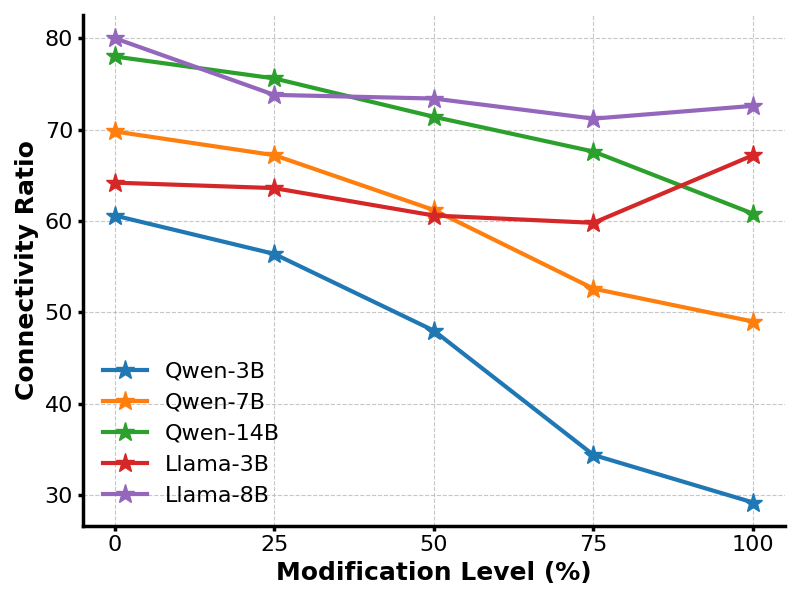
\includegraphics[width=\linewidth]{figures/connect.png}
        \vspace{-0.5em}
        %\caption{Connectivity Ratio v.s. Modification Level}
        \label{fig:c_vs_mod}
    \end{subfigure}
    \hfill
    \begin{subfigure}{0.33\textwidth}
        \centering
        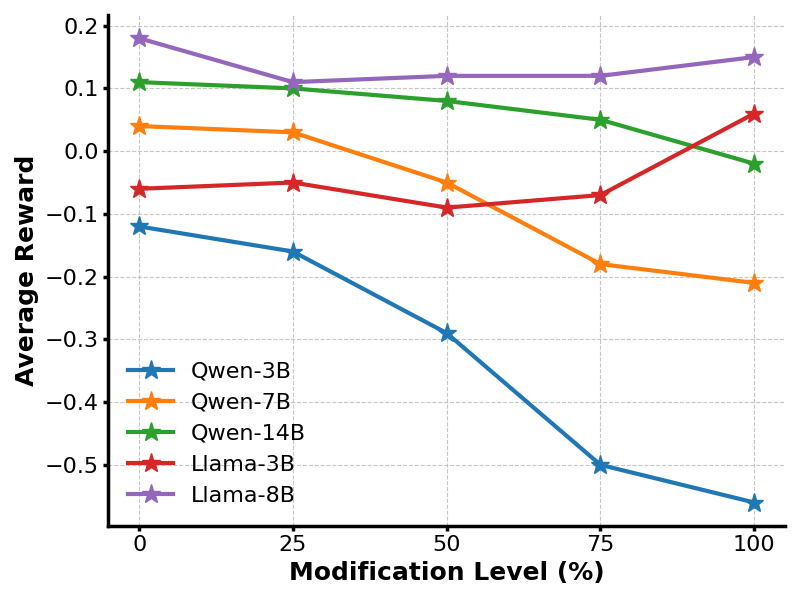
\includegraphics[width=\linewidth]{figures/reward.png}
        \vspace{-0.5em}
        %\caption{Average Reward v.s. Modification Level}
        \label{fig:f1_vs_mod}
    \end{subfigure}
    \hfill
    \begin{subfigure}{0.33\textwidth}
        \centering
        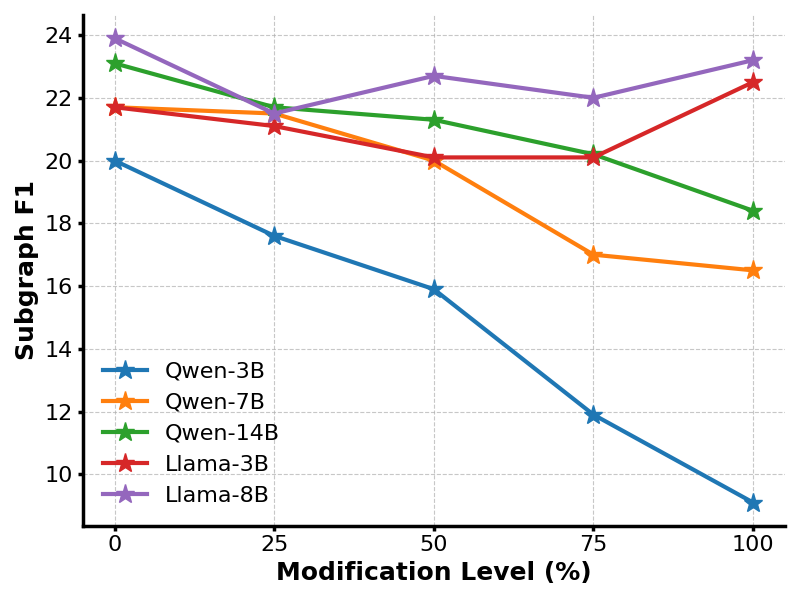
\includegraphics[width=\linewidth]{figures/f1.png}
        \vspace{-0.5em}
        %\caption{Subgraph F1 v.s. Modification Level}
        \label{fig:r_vs_mod}
    \end{subfigure}
    \vspace{-2em}
    \caption{Comparison of connectivity ratio, average reward, and subgraph F1 under different modification levels in MetaQA.}
    \label{fig:comparison_generalization}
    \vspace{-0.8em}
\end{figure*}


To examine the robustness and transferability of \textit{UniRel}, we evaluate its ability to generalize across datasets.
Table~\ref{tab:generalization_results} reports partial generalization results, with the complete results provided in Appendix~\ref{sec:generalization_results_details}.
Specifically, UniRel is trained on the largest dataset, DBpedia500, and directly evaluated on the remaining datasets without additional training.

\textbf{Settings.} \textbf{\emph{Original}} denotes the standard setting, where datasets retain their original entity and relation names.
\textbf{\emph{Modified}} denotes a controlled variant in which all entities and relations are replaced with random identifiers (e.g., $\text{ENT}1,\dots,\text{ENT}n$, $\text{REL}1,\dots,\text{REL}m$), thereby removing semantic cues while preserving graph structure.

\textbf{Result Analysis.} As shown in the \emph{Original} rows, the models are able to generate valid subgraphs even for previously unseen entities and relations, demonstrating a notable degree of cross-domain transferability.
Compared with the Prompting results in Table~\ref{tab:main_results}, these models achieve substantially higher performance across all metrics, often approaching the connectivity, average reward, and Subgraph F1 of their in-domain UniRel counterparts, suggesting that UniRel generalizes effectively beyond the training domain.

% This observation motivates the hypothesis that LLMs exploit semantic regularities acquired during training to generalize to novel patterns.
% To test this hypothesis, we evaluate UniRel under the \emph{Modified} setting.

This motivates the hypothesis that LLMs leverage semantic regularities to generalize.
We test this by evaluating UniRel under the \emph{Modified} setting.
% This observation motivates the hypothesis that LLMs can exploit semantic regularities acquired during training to generalize to novel patterns.  
% To test this, we construct \emph{Modified} versions of each dataset by replacing all entities and relations with random identifiers (e.g., $\text{ENT}1,\dots,\text{ENT}n$, $\text{REL}1,\dots,\text{REL}m$), thereby eliminating semantic cues.

As expected, the \emph{Modified} rows exhibit a substantial performance drop across all datasets for the Qwen family, highlighting the critical role of semantic information in enabling cross-domain transfer.
In contrast, the Llama family is less affected: the 3B model shows only marginal changes, and although the 8B model does experience performance degradation, the magnitude remains considerably smaller than that observed for Qwen models.
For example, on YAGO3-10, Qwen-3B suffers reductions of \textbf{58.3\%} in connectivity ratio, \textbf{266.67\%} in average reward, and \textbf{37.13\%} in Subgraph F1, whereas Llama-3B shows much smaller changes of \textbf{0.45\%}, \textbf{13.89\%}, and \textbf{3.96\%}, respectively.
Overall, these results indicate that Qwen models are more sensitive to the removal of semantic information than Llama models.


To further probe this effect, we conduct an additional experiment on MetaQA, where a fraction of entities and relations are replaced with random identifiers.
We consider partial modifications at 25\%, 50\%, and 75\%, thereby progressively diminishing the amount of preserved semantic information.
As shown in Figure~\ref{fig:comparison_generalization}, Qwen models exhibit a consistent degradation in connectivity ratio, average reward, and Subgraph F1 as the modification level increases, indicating that both feasibility and structural quality of the generated subgraphs strongly depend on semantic regularities in the knowledge graph.
By contrast, Llama models are less affected: the 3B variant shows only minor fluctuations, with a slight initial decline followed by a modest recovery, whereas the 8B model exhibits a mild downward trend, with reductions of \textbf{9.25\%} in connectivity ratio, \textbf{16.67\%} in average reward, and \textbf{2.93\%} in Subgraph F1 between the original and fully modified settings.

Taken together, these findings suggest that Qwen models rely more on semantic information for cross-dataset generalization, whereas Llama models draw more on structural connectivity to sustain stable performance. 





\vspace{-0.5em}
\subsection{Scalability}
\begin{table*}[t]
\centering
\caption{Performance comparison of Prompting and UniRel on DBpedia50 across three-entity and four-entity queries.}
\resizebox{0.9\textwidth}{!}{%
\begin{tabular}{ll|cccc|ccccc}
\toprule
\multicolumn{2}{c|}{\textbf{Models}}
 & \multicolumn{4}{c|}{\textbf{Three Entities}} 
 & \multicolumn{5}{c}{\textbf{Four Entities}} \\ 
\multicolumn{2}{l|}{} 
 & \makecell{Full Conn. } 
 & \makecell{Pairwise Conn.} 
 & {Reward} 
 & {F1} 
 & \makecell{Full Conn.} 
 & \makecell{Triple Conn.} 
 & \makecell{Pairwise Conn.} 
 & {Reward}
 & {F1} \\ 
\midrule 
\multirow{2}{*}{Qwen3B} 
 & Prompting    & 4.2\% & 2.2\% & -1.21 & 6.9 & 1.8\% & 0.0\% & 0.6\% & -2.31 & 2.5 \\
 & UniRel  & 69.2\% & 17.2\% & 1.17 & 44.6 & 8.2\% & 18.6\% & 50.8\% & -0.29 & 35.2\\

\multirow{2}{*}{Qwen7B} 
 & Prompting    & 10.4\% & 6.6\% & -0.66 & 18.6 & 5.2\% & 2.0\% & 4.8\% & -0.84 & 12.1\\
 & UniRel  & 73.4\% & 18.0\% & 1.27 & 45.5 & 55.4\% & 16.4\% & 18.0\% & 0.78 & 43.7\\

\multirow{2}{*}{Qwen14B} 
 & Prompting    & 13.8\% & 13.6\% & -0.56 & 29.3 & 4.8\% & 0.6\% & 5.6\% & -2.37 & 22.0 \\
 & UniRel  & 95.4\% & 2.0\%  & 1.59 & 50.0 & 83.2\% & 6.1\% & 4.3\% & 1.26 &  46.9\\ 
\midrule

\multirow{2}{*}{Llama3B} 
 & Prompting    & 0.0\% & 0.0\% & -2.93 & 0.0   & 0.0\% & 0.0\% & 0.0\% & -3.82 & 0.0\\
 & UniRel  & 90.8\% & 7.6\% & 1.57 & 50.2  & 48.4\% & 18.4\% & 24.2\% & 0.68 & 43.9\\

\multirow{2}{*}{Llama8B} 
 & Prompting    & 0.0\% & 0.0\% & -2.90 & 0.0 & 0.0\% & 0.0\% & 0.0\% & -3.78 & 0.0 \\
 & UniRel  & 94.6\% & 4.8\% & 1.61 & 51.1 & 80.0\% & 5.6\% & 10.2\% & 1.26 & 46.8\\

\midrule
\rowcolor{blue!10}
\multicolumn{2}{l|}{\textbf{Optimal Reward}} & \multicolumn{4}{c|}{1.74} & \multicolumn{5}{c}{1.63} \\
\bottomrule
\end{tabular}}
\vspace{-1em}
\label{tab:multi_entity_results}
\end{table*}

To assess the scalability of \textit{UniRel}, we extend our evaluation from two-entity queries to queries involving three and four entities on the DBpedia50 dataset.
Unlike the two-entity case, where connectivity is measured by a \emph{connectivity ratio}, multi-entity queries allow for a richer characterization.

For three-entity queries, we report both the \emph{pairwise connectivity ratio} (the percentage of queries where \textit{only} two entities are connected) and the \emph{full connectivity ratio} (all three entities are connected).
For four-entity queries, we distinguish three levels: (i) \emph{pairwise connectivity ratio}, (ii) \emph{triple connectivity ratio}, and (iii) \emph{full connectivity ratio}.


Table~\ref{tab:multi_entity_results} summarizes the performance of Prompting and UniRel on DBpedia50 across three-entity and four-entity queries.
Across both settings, Prompting models exhibit limited ability to recover valid subgraphs.
By contrast, UniRel demonstrates substantial generalization gains: for three-entity queries, the full connectivity ratio increases by \textbf{591.3\%}, the average reward by \textbf{277.27\%}, and the Subgraph F1 by \textbf{70.65\%};
for four-entity queries, the corresponding gains reach \textbf{355.6\%} in full connectivity, \textbf{87.5\%} in reward, and \textbf{113.1\%} in Subgraph F1.
Importantly, even when full connectivity is not achieved, UniRel consistently improves pairwise and triple connectivity ratios together with Subgraph F1, indicating its ability to recover meaningful partial structures that explain subsets of entity relations.
Moreover, Llama models consistently outperform Qwen models, in some cases approaching the optimal reward, highlighting their stronger capacity to leverage structural information in multi-entity reasoning.

These findings collectively demonstrate the scalability of the proposed framework to more complex multi-entity scenarios and underscore its applicability to real-world KGQA tasks that involve reasoning over multiple entities. 


% \begin{table}[h]
% \centering
% \caption{Performance Comparison with RL-tuned LLM}
% \begin{tabular}{lcccc}
% \toprule
% \textbf{Model} & \textbf{Configuration} & \textbf{Hit@1} & \textbf{F1} \\
% \midrule
% \multirow{2}{*}{G-retriever} & Base & 70.49 & 53.41 \\
%  & Retriever + RL-tuned & 70.10 & \textbf{58.90} \\
% \midrule
% \multirow{2}{*}{ROG} & Base & \textbf{85.70} & 70.80 \\
%  & Retriever + RL-tuned & 79.00 & \textbf{72.30} \\
% \midrule
% \multirow{2}{*}{KAPING} & Base & 52.64 & - \\
%  & Retriever + RL-tuned & 71.40 & 61.70 \\
% \midrule
% \multirow{2}{*}{GNN} & Base & 80.60 & \textbf{71.30} \\
%  & Retriever + RL-tuned & 80.40 & 70.90 \\
% \midrule
% \multirow{2}{*}{GNN-RA} & Base & 82.80 & 73.50 \\
%  & Retriever + RL-tuned & 82.50 & \textbf{77.00} \\
% \bottomrule
% \end{tabular}
% \end{table}

\begin{table}[t]
\centering
\caption{Comparison results for entity-centric KGQA.}
\resizebox{0.5\textwidth}{!}{%
\begin{tabular}{llcccc}
\toprule
\multirow{2}{*}{Retriever} & \multirow{2}{*}{Pipeline}
& \multicolumn{2}{c}{WebQSP} & \multicolumn{2}{c}{CWQ} \\
\cmidrule(lr){3-4} \cmidrule(lr){5-6}
& & Hit@1 & F1 & Hit@1 & F1 \\
\midrule
PCST (G-retriever) & Original & 70.49 & 53.41 & -- & -- \\
~\cite{he2024g}    & UniRel   & \textbf{70.50} & \textbf{58.90} & 49.53 & 44.70 \\
\midrule
KAPING Retriever   & Original & 52.64 & -- & -- & -- \\
~\cite{baek2023knowledge}  & UniRel   & \textbf{72.00} & 61.40 & 50.40 & 46.20 \\
\midrule
ROG Retriever      & Original & \textbf{85.70} & 70.80 & \textbf{62.60} & 56.20 \\
~\cite{luo2024reasoning}& UniRel   & 80.00 & \textbf{72.30} & 59.2 & \textbf{57.20} \\
\midrule
GNN Retriever      & Original & \textbf{80.60} & \textbf{71.30} & 61.70 & 59.40 \\
~\cite{mavromatis2024gnn} & UniRel   & 80.20 & 71.10 & \textbf{65.20} & \textbf{61.70} \\
\midrule
GNN-RA Retriever   & Original & \textbf{82.80} & 73.50 & 62.80 & 62.40 \\
~\cite{mavromatis2024gnn} & UniRel   & 82.70 & \textbf{77.10} & \textbf{66.50} & \textbf{63.70} \\
\bottomrule
\end{tabular}
}
\label{tab:entity_centric}
\vspace{-1em}
\end{table}


\subsection{UniRel for Entity-Centric KGQA}
Although UniRel is designed for relation-centric KGQA, its pipeline is task-agnostic and can be readily adapted to conventional entity-centric KGQA.
Specifically, we replace the subgraph retriever module with task-specific entity-centric retrievers, while keeping the remaining reasoning and generation components unchanged.

We instantiate this adaptation using retrievers from prior work, and all models use LLaMA2-7B-chat~\cite{touvron2023llama} as the base LLM.
Evaluation is conducted on  WebQSP~\cite{yih2016value} and CWQ~\cite{talmor2018web} using standard Hit@1 and F1 metrics. More details are provided in Appendix~\ref{sec:entity_centric_results_details}.

% As shown in Table~\ref{tab:entity_centric}, under the same retriever, replacing the original reasoning component with the UniRel pipeline yields competitive and often improved performance, demonstrating that UniRel can be effectively applied to entity-centric KGQA.

% Table~\ref{tab:entity_centric} reports the results of applying the UniRel pipeline to entity-centric KGQA under different retrievers.
% For each retriever, we compare UniRel with the original pipeline from prior work under the same retriever and base LLM, showing consistent F1 improvements and competitive or improved Hit@1 scores.
% Table~\ref{tab:entity_centric} reports results of applying UniRel to entity-centric KGQA under different retrievers.
% For each retriever, we compare UniRel with the original pipeline reported in prior work under the same retriever and base LLM, showing consistent F1 improvements and competitive or improved Hit@1 scores.
Table~\ref{tab:entity_centric} reports the results of applying the UniRel pipeline to entity-centric KGQA under different retrievers. For each retriever, we compare the original pipeline with UniRel while keeping the retriever and base LLM fixed. The results of the original pipelines are taken directly from the prior work. Overall, UniRel consistently improves F1 across most settings and achieves competitive or improved Hit@1 scores.
Notably, under PCST and KAPING retrievers, UniRel substantially improves F1 on WebQSP, indicating more complete answer coverage.
For stronger retrievers such as GNN and GNN-RA, UniRel yields consistent gains on both WebQSP and CWQ, suggesting that improved relational reasoning can further benefit entity-centric QA when high-quality subgraphs are available.


